\documentclass[11pt]{jarticle}
\usepackage{ITCannual}
\usepackage{amsmath}
\usepackage{amssymb}
\usepackage{times}
\usepackage{graphicx}

%\usepackage[style=numeric]{biblatex}

\title{データ科学研究部門 研究報告}
\author{小林, 松島, 姜, 川瀬}

\begin{document}
\maketitle

\section{前年同様、各部門自由記述}
...

\section{データ科学部門の研究活動}

\subsection{研究報告(小林 博樹)}


\subsection{研究報告(松島)}
本節では松島研究室の研究活動について報告する。
2019年度および2020年度に、弊研究室では解釈可能な機械学習手法の効率的な計算手法についての研究を推進してきた。

大量のデータから複雑な関数を推定することにより画像データや言語データを予測したり生成したりするなど、表層的に駆使することは可能になってきた。
しかしながら我々の画像や言語に対する理解が進んだわけではない。現代社会には様々なデータがあり、データを上記の意味で駆使するだけでなく、データの隠れた法則性や生成原理などの理解に結び付く属性間の関係を抽出することが求められる。

機械学習は予測や分類など表層的なデータの駆使の方法論であるだけでなく、
データの関係を明らかにして人間の理解を助けるための方法論でもあり、
特にデータ保持者の目線に立った機械学習の手法の研究を行ってきた。
成果は主に以下の3分野に大別される。
\begin{itemize}
    \item 一般化加法モデルに関する研究
    \item 組合せ線形モデルに関する研究
    \item 部分空間クラスタリングに関する研究
\end{itemize}

一般化加法モデルと組み合わせ線形モデルは
属性間の線形な関係を越えて、非線形な関係を抽出するための枠組みである。
部分空間クラスタリングはデータ集合が持つ単純な線形関係を超えて、
データのクラスタリングを行ってそれぞれのクラスタが持つ線形関係を抽出する枠組みである。


\subsubsection{一般化加法モデルに関する研究}
教師あり学習の文脈において、線形モデルの学習とは以下のようにあらわされるデータの属性間の線形な関係を抽出する枠組みととらえることができる:
\begin{align*}
    y = \sum_{j=1}^d w_j x_j.
\end{align*}
データの属性$y$は通常予測したい変数であり、
予測のために用いられるデータの他の属性が$x_j$であらわされる($j=1,\ldots,d$)。与えられたデータ集合を用いて各$w_j$は実数全体から推定される。
一般化加法モデル\cite{F}は線形モデルと同様に以下のような関係を抽出する枠組みである:
\begin{align*}
    y = \sum_{j=1}^d f_j (x_j).
\end{align*}
このとき、与えられたデータ集合を用いて各$f_j$は(十分広い)関数クラス$F$から推定される。
このような$f_j$を推定できれば、例えば年齢と収入の非線形な関係などがデータから学習できると考えられる。

最も単純な手法は$F$を推定の簡単さのために狭めの関数クラスに制限することである。一般に与えられた基底関数集合$\left\{\varphi_k:\mathbb{R} \to \mathbb{R} \right\}_{k=1,\ldots,K}$に対し
\begin{align*}
  F=\left\{  \sum_{j=1}^d\sum_{k=1}^{d’} w_{kj}\varphi_k(x_j) \right\}
\end{align*}
とすれば、通常の線形モデルの学習と同様に学習が可能であるが、
基底関数たち$\phi_k$と$d'$をデータに応じてうまく選ぶ必要がある。このような方法はパラメトリックな手法と呼ばれる。

利用可能なデータ数に応じて関数クラスの大きさが変わる。
具体的にはデータ数が大きくなれば関数クラスも広くなっていくような手法をノンパラメトリックな手法と呼ぶ。
ノンパラメトリックな手法では各$f_j$は以下のように表される無限次元の空間$F$から推定されると考えることができる:
\begin{align*}
    F = \{f | \|f\|\le C\}
\end{align*}
ここで$\|\cdot\|$はある関数空間上で定義されたノルムある。上述のような手法はカーネル法を使うよりなかった。
我々の手法はカーネル法よりも効率的に学習が可能である。

さらに対象の属性が二変数関数$f_{j,k}(x_j,x_k)$の和で表されるような複雑な関係性をデータから学習して可視化することを考える。すなわち、以下の以下のような$y$と$x$の関係を抽出することを考える:
\begin{align*}
    y = \sum_{j,k} f_{j,k} (x_j,x_k)
\end{align*}
ここでデータから$f_{j,k}$を$F$から推定する。
\cite{KM01}、\cite{KM02}では二変数関数の空間に対して
二変数全変動ノルムを新しく定義し、これに基づく定式化および推定のための最適化アルゴリズムを提案した。さらに計算機実験において既存手法に比べより正確に真の関数を推定できることを示した。
\begin{figure*}[h]
    \centering
    \begin{tabular}{c}
        \begin{minipage}{0.04\hsize}
            \centering
        \end{minipage}
        \begin{minipage}{0.24\hsize}
            \centering
            Ground Truth
        \end{minipage}
        \begin{minipage}{0.24\hsize}
            \centering
            Proposed
        \end{minipage}
        \begin{minipage}{0.24\hsize}
            \centering
            $\rm GA^2M$
        \end{minipage}
        \begin{minipage}{0.24\hsize}
            \centering
            pyGAM
        \end{minipage}
        \\ \hline
        \begin{minipage}{0.04\hsize}
            \small
            $x_0, x_1$
        \end{minipage}
        \begin{minipage}{0.24\hsize}
            \centering
            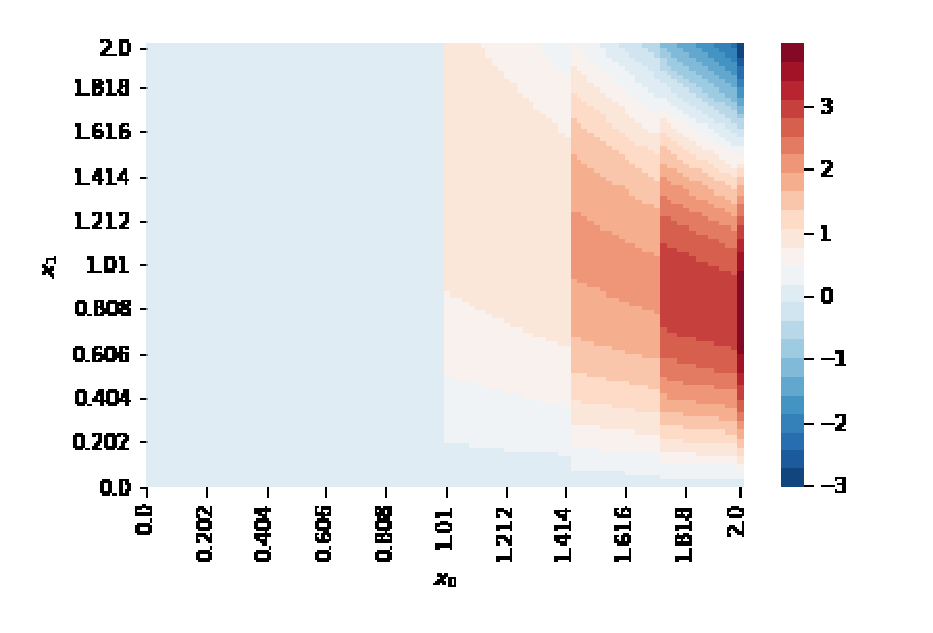
\includegraphics[width=0.95\hsize]{Matsushima/heatmaps/ideal-01.eps}
            % 理論値:$x_0 x_1$
        \end{minipage}
        \begin{minipage}{0.24\hsize}
            \centering
            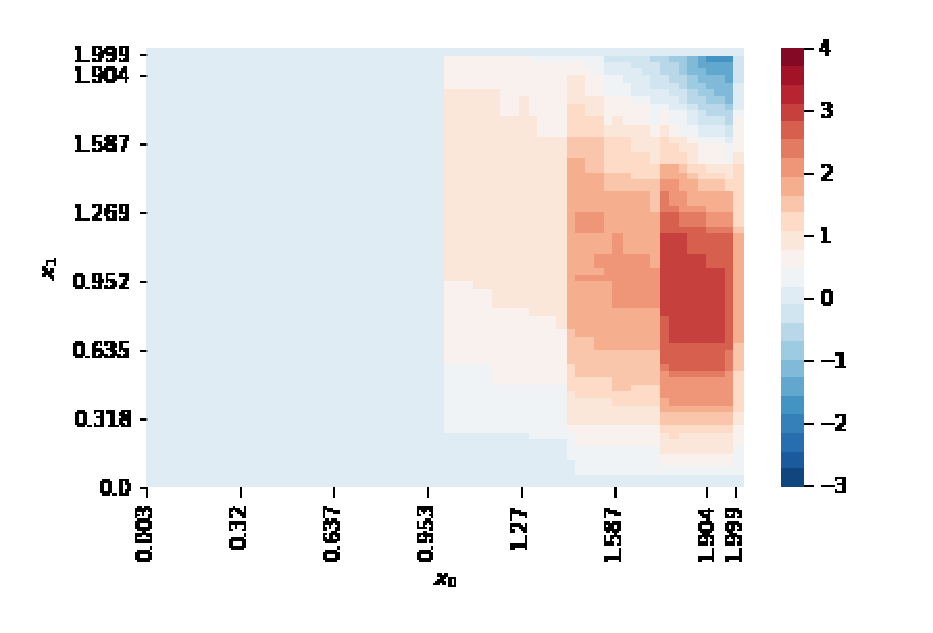
\includegraphics[width=0.95\hsize]{Matsushima/heatmaps/tvgam-01.eps}
            % IGAMの学習した相互作用
        \end{minipage}
        \begin{minipage}{0.24\hsize}
            \centering
            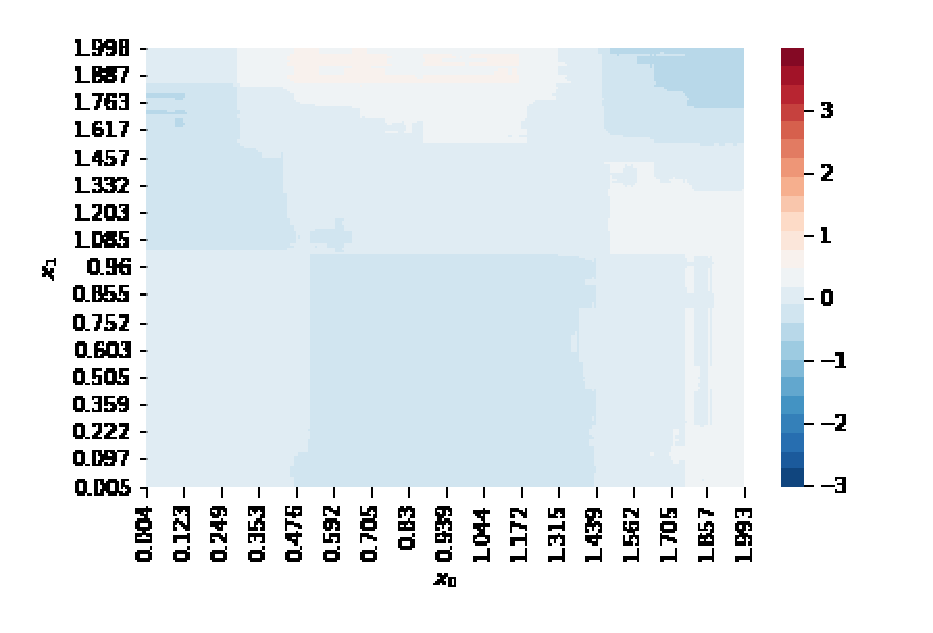
\includegraphics[width=0.95\hsize]{Matsushima/heatmaps/mltk-01.eps}
            % $\rm GA^2M$の学習した相互作用
        \end{minipage}
        \begin{minipage}{0.24\hsize}
            \centering
            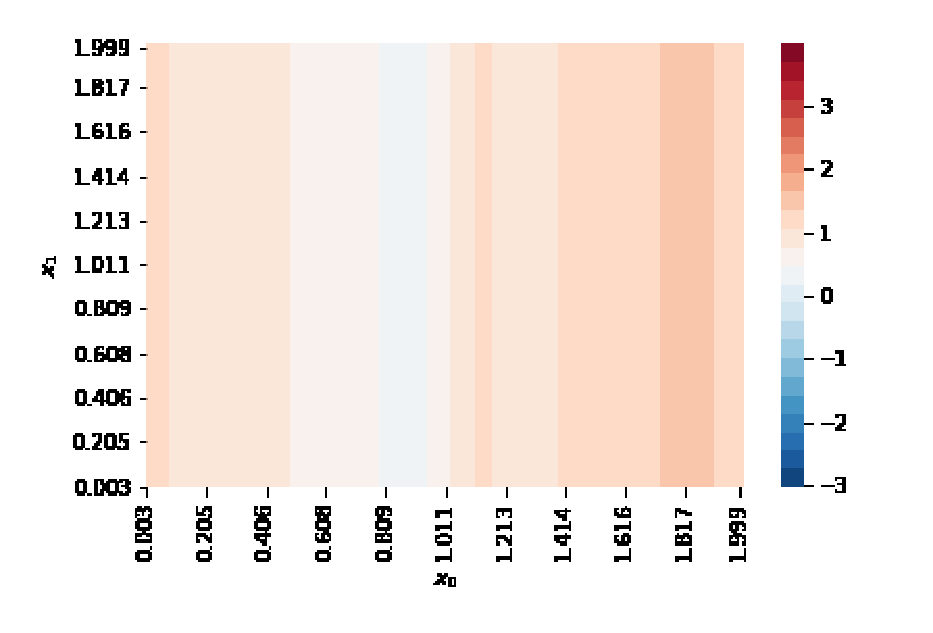
\includegraphics[width=0.95\hsize]{Matsushima/heatmaps/pygam-01.eps}
        \end{minipage}
    \end{tabular}
    \caption{人口データを用いた提案手法と既存手法($\rm GA^2M$およびpyGAM)の推定した二変数相互作用を表す関数の様子。Ground Truthは訓練データを生成した真の関数。}
\label{fig:heatmap-comparison-synthetic-data-2}
\end{figure*}

\subsubsection{組合せ線形モデルに関する研究}

組合せ線形モデルでは離散データ集合を考える。
実用的なデータの属性は例えば性別など示量的に表せないことも多く、このような属性の集合は通常離散データ、すなわち$\{0,1\}^n$上のデータとして扱われることが多い。
このよ8うな離散的な属性を複数持つようなデータを考えると、属性間の相互作用の数はデータの属性数に対して指数的に増加するため、離散データ空間での相互作用を扱う効率的な学習方法を発明することは重要である。

 前述の目的のためにイジングモデルやボルツマンマシンのような無向グラフィカルモデルと言われるモデルがよく用いられる。これらのモデルは二次までの相互作用しか扱えないのに対して、高次元対数線形モデルはデータ間のより高次元の相互作用を表現することが可能である。また、高次元対数線形モデルはフィッシャー情報量とe-接続とm-接続に基づく双対平坦構造を持つことから、理論的にも重要である。
 
高次対数線形モデルは
\begin{align*}
    \log P(x;\theta) = \sum_{\phi\in B} \theta_\phi \phi(x)  - \log\left( \sum_{x'\in S} \exp\left( \sum_{\phi\in B} \theta_\phi \phi(x') \right) \right)    
\end{align*}
と表される。ここで$\phi \in B \subset \{0,1\}^n$と$\phi:\{0,1\}^n\to \{0,1\} $を同一視する。すなわち$\phi(x)$の値を以下で定義する。
\begin{align*}
    \phi(x)  = \begin{cases}
    1 & 全ての j で \phi_j \le x_j, \\
    0 & 上記以外.
    \end{cases}
\end{align*}

\cite{LMY01}では、識別モデルにおいて教師あり学習を行う場合に効率的な学習アルゴリズムを提案した。実験によって論理結合による特徴は各説明変数が同時に真である場合の効果を表すと解釈できるため、解釈性も予測性能も高い予測が可能であることを示した。
行う。

さらに本研究では生成モデル、すなわち二値データの分布の推定問題も対象とした。教師なし学習の文脈では、与えられたデータの特徴を解釈可能であり、かつ真の分布をよく近似する分布を推定することを目指す。
本研究では自然スパース性(Natural Sparsity, Natural Sparseness)という概念を導入し、より自然スパース性が高いモデルを推定するような定式化と方法論を提案する。

$S\subset\{0,1\}^n$に関して真の確率分布は以下の集合$M$の元であるとする。
\begin{align*}
    M = \left\{ P(\cdot)\middle| 0<P(x)<1, \sum_{x\in S} P(x) = 1 \right\}
\end{align*}
$M$には双対平坦な座標系が存在し、それぞれの座標系での値を
自然パラメータ$\theta \in \mathbb{R}^{|S|}$
と期待パラメータ$\eta \in \mathbb{R}^{|S|}$で表す。
この時、任意の分布に関して$\eta$はスパースでない。
一方で$\theta$は非零要素を多く含むものは単純な分布とされており、
例えば単純な対数線形モデルやイジングモデルは高次の$\theta$の値を0に制限したモデルである。

さらに自然パラメータは$\theta \in \mathbb{R}^{2^n}$へ拡張できる。
この時一つの分布$P$に対しいくつかの$\theta$が対応し、スパースネスの値も表現の仕方によって変わる。(例を挙げる)
このように考えると、自然スパース性は以下のように定義することが望ましい。

\cite{HSM01}、\cite{HSM02}ではこのような意味でスパースなモデルの学習が座標降下法により効率的に学習可能であることを示した。


\subsubsection{部分空間クラスタリングに関する研究}

部分空間クラスタリングとは複数の低次元空間にデータをクラスタリングする手法である。通常のクラスタリング手法では距離的に近いデータの集まりをクラスタとみなす。一方で、部分空間クラスタリングでは同じ低次元空間にあるデータをクラスタとみなす(図~\ref{fig:my_label}を参照)。画像データや文章データなどはタスクによって部分空間クラスタリングをした方がよいということが2011年VIDAL\cite{SC}によって提案されて以降、多くの部分空間クラスタリング手法が開発されている。

\begin{figure}[h]
    \centering
    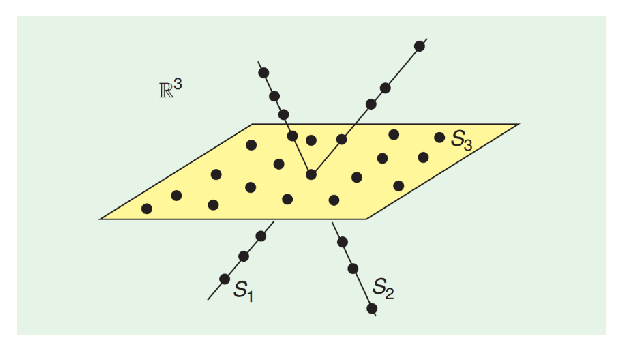
\includegraphics[width=7cm]{Matsushima/sc.eps}
    \caption{部分空間クラスタリングの3次元の例(\cite{SC}から抜粋)。距離が近い点同士ではなく、同じ平面上もしくは同じ直線上(部分空間上)にある点同士をクラスタとみなす。}
    \label{fig:my_label}
\end{figure}
\cite{NM01}は〜

\begin{thebibliography}{9}
\bibitem{F}
    Friedman, J., Hastie, T., & Tibshirani, R. (2010). 
    Applications of the lasso and grouped lasso to the estimation of sparse graphical models (pp. 1-22). Technical report, Stanford University.
\bibitem{SC}
 VIDAL, René. Subspace clustering. IEEE Signal Processing Magazine, 2011, 28.2: 52-68.
\end{thebibliography}



\subsection{研究報告(姜 仁河)}
モノのインターネット(IoT)、ビッグデータ、人工知能技術の急速な発展に伴い、スマートシティは新しい研究分野として政府や産業界から非常に重視されている。様々なマルチモーダルの人の流れ移動データと都市のビッグデータ(スマートフォン位置データ、携帯電話の通話記録データ、GPS 軌跡データ、都市交通網データ、自然災害データ、伝染病データ、公共健康データなど)を統合、処理、分析し、新世代の人工知能技術(深層学習、強化学習、アンサンブル学習など)と結び付け、都市規模の人の流れの移動についてのモデリング、シミュレーション、予測を実現することにより、都市の交通整理、都市における緊急事態管理、災害時の人道支援、伝染病の拡大予防対策、公共の健康促進などの実現を目指す。これを背景にし、2019年度および2020年度に、引き続き私はデータ駆動型知能とアーバンコンピューティングについて研究活動を行ってきた。お陰様で複数の研究成果\cite{JIANG1901,JIANG2001,JIANG2002,JIANG2003,JIANG1902,JIANG1903,JIANG1904,JIANG2004,JIANG2005,JIANG2006}をあげている。ここにて以下2点の研究プロジェクトをピックアップして詳しく紹介する。

\begin{itemize}
    \item 深層学習による都市全体の群衆密度・流れの予測
    \item モビリティデータと医療データを統合したインフルエンザ流行の解析・予測
\end{itemize}

\subsubsection{深層学習による都市全体の群衆密度・流れの予測}
大規模な都市区域を数々のきめ細かいメッシュグリッドへとメッシングすることで、連続的な期間における都市全体の群集や交通情報を映像のように表現し、各タイムスタンプを一枚の映像フレームとして扱うことができる(図\ref{fig:intro1_jiang})。この考え方に基づき、都市全体の群集や交通に関する映像型の予測に対応するため一連の手法が提案された。現在、この手法群の評価は (1) 一部のモデルは他のモデルと比較できない、(2) 一部のモデルは群集流動データではなくタクシーや自転車などの交通流量のみによって検証されている、(3) 一部のモデルは天候データやPOIデータなどの外部データ源を活用している、(4) 一部のモデルは独自に設計したオブジェクト関数を用いている、(5) ホットステーションや朝の混雑時間における住宅地域といった一部の具体的な地域や時間帯によるケーススタディが欠けている、といった観点から未だに不十分である。本研究を通じ、我々は実世界のスマートフォンによるアプリケーションを通じて生成した集合的な人の移動に関する新たなデータセットを公開し、複数のオープンデータセットに基づいてそのような種類のアーバンコンピューティング問題に対する標準的なベンチマークを構築することを試みる。具体的には、(1) 群集および交通の密度予測、流出入予測といった2種類の古典的な問題を対象として設定する。前者では次のタイムスタンプにおいて各メッシュグリッドに何人または何台いるかを予測し、後者では次の時間間隔において各メッシュグリッドに何人または何台が流入または流出するかを予測する。過去に観察した複数ステップ分のデータを入力として扱い、次のステップにおける予測結果を出力として報告する。(2) 広く普及しているスマートフォンのアプリによるGPSログデータを用いて実世界の群集密度や流動を反映する新規データセットを作成する。次に、作成した新規データセットと既存のデータセットを用いて群集および交通の予測を実施できる。(3) 統一した目的関数であるMSEをモデルの訓練に採用し、外部データ源や関連する処理モジュールをモデルから除外する。それにより、時空間データの映像型モデリングに関する純粋な能力を公平に検証することができる。(4) 選択した地域の時系列の予測結果をケーススタディとして追加し、異なる場所や時間に対する有効性を実証する。
\begin{figure}[h]
	\centering	
	\includegraphics[width=0.95\textwidth]{Kyo/figure/intro1.eps}
	\caption{都市全体の群集密度や流れは映像のように表現}
	\label{fig:intro1_jiang}
\end{figure}

\subsubsection{モビリティデータと医療データを統合したインフルエンザ流行の解析・予測}
インフルエンザの流行により、健康被害や社会経済への影響が大きいため、インフルエンザがいつどこで発生し、感染がどのように拡大するかは重要な課題として政府や自治体に強調された。ビッグデータ時代、特にIoT(Internet of Things)時代に、従来の医学・免疫学分野になかったデータ駆動の方法を利用し、インフルエンザ流行のメカニズムを解明する。さらにそのメカニズムに基づいて流行状況の高精度な予測モデルを構築する。具体的に、本研究はブログウォッチャーGPS軌跡データ(人の移動モビリティデータとNDBレセプトデータ(医療データ)を利用する。ブログウォッチャーGPS軌跡データとは、提携アプリをダウンロードし、位置情報の取得を許可したユーザーのスマートフォン端末から、GPSで補足した経度緯度の位置情報である。一方、NDBレセプトデータとは、情報データベース(NDB)に蓄積されたレセプト情報・薬の処方情報などであり、インフルエンザ感染数のproxyとなるデータでもある。この二つのデータを組み合わせて、過去十年間の感染の広がり方の差異と人的空間移動の状況を解析し、まず地域間の人の移動がインフルエンザ感染・流行に寄与しているかを検証する;そして、関連していることが確定されればその人の移動によるインフルエンザ流行のメカニズムに基づき、リアルタイムかつ高精度のインフルエンザ流行状況の予測モデルを構築する。なお、本研究について、1)データへのアクセス(個人情報などの課題);2)データの粒度の違い、仕様の違い;3)データ量の多さ;4)モデリング手法などのチャレンジを克服するために、GPS軌跡データとNDB医療データを同時に用意するだけでなく、それぞれのデータに高度な解析能力を持つ時空間データ専門家及び医療データ専門家の高度なコラボレーションも欠かせない。異分野のデータと異分野の専門知識を備えた上で、次世代の人工知能技術(深層学習、強化学習、アンサンブル学習など)に基づき、新型のデータ統合解析技術・AI予測モデルを開発する。本研究内容の概要は以下の図\ref{fig:intro2_jiang}にまとめている。

\begin{figure}[h]
	\centering	
	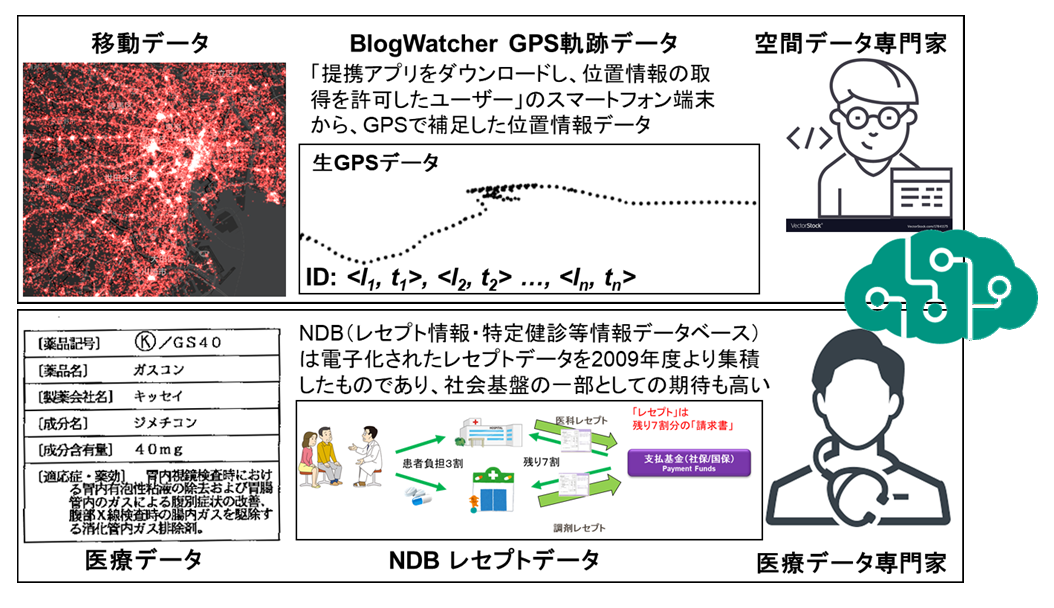
\includegraphics[width=0.95\textwidth]{Kyo/figure/intro2.eps}
	\caption{モビリティデータと医療データの統合解析}
	\label{fig:intro2_jiang}
\end{figure}
\subsection{野生動物ワイヤレスセンサネットワーク実証実験基盤構築に向けた研究(川瀬)}
\subsubsection{概要}
インフラ基盤のない野生環境下での運用を想定した野生動物装着型ワイヤレスセンサネットワーク(WSN)の開発を念頭に、放牧下の家畜動物による効率的な評価実験基盤の構築を目指している。2020年度は国内の放牧場に協力を依頼し、実験基盤の構築・設置、現地での評価実験実施を目指して進めてきたが、コロナ禍により中断している。また野生動物装着型WSNに特化したデータ共有手法について検討を進めている。
\subsubsection{背景}
インフラ基盤のない野生環境化において、個々の野生動物にモバイルセンサを運搬してもらう野生動物装着型WSNは様々な活用が可能であると考えられている。例えば、有害鳥獣類対策・感染症伝播経路特定・人間が容易に侵入することができない区域での空間情報の収集に役立てることができる。しかし、インフラ未整備区域での評価実験の実施は多くのコストが必要になるため、繰り返し実験が可能な“放牧下の家畜動物”による効率的な評価実験基盤の構築を目指す。
\subsubsection{内容}
放牧下の家畜動物たちがモバイルセンサを持ち歩き、単独行動時に取得したデータを集団行動時に共有する。そして最終的にシンクノード付近に滞在する個体からデータを回収し、モバイル通信を介して遠隔地でデータを蓄積・リアルタイムでの分析を一体的に試みることを目指す。既に、野生動物装着型WSNを見据えた動物装着モバイルセンサノードの開発・実験、モバイル通信による広域データ収集基盤の試運転を行ってきた。そこで、本研究では放牧場及び放牧家畜の協力のもと、一体的な評価実験基盤の構築及び評価実験を実施する。
\subsubsection  {成果報告}
本研究は、2020年度国立情報学研究所公募型共同研究として進められた。北海道安平町や岩手県久慈市などの肉牛放牧場らと実験基盤の構築・設置、現地での評価実験実施の交渉を行っていたが、コロナ禍により中断している。また、野生動物装着型WSNでは、いつ・どの組み合わせで発生するかわからない野生動物同士の遭遇を考慮したうえで、無線通信での効率的かつ精確なデータ共有手法が必要になる。そこで、このデータ共有手法について検討を進めている。


\section{成果要覧}

\begin{招待講演}{1}

\end{招待講演}

\begin{招待論文}{1}

\end{招待論文}

\begin{受賞}{1}

\end{受賞}

\begin{著書}{1}

\end{著書}

\begin{雑誌論文}{1}

\bibitem{AA10}
AA:
AAのジャーナル,掲載誌名,巻,号,ppXX-YY,年月
\end{雑誌論文}

\begin{査読付}{1}

\bibitem{HSM02}
S. Hayashi, M. Sugiyama, S. Matsushima: “Coordinate Descent Method for Log-linear Model on Posets,”  In Proceedings of IEEE International Conference on Data Science and Advanced Analytics (DSAA), pp. 99-108 (2020)
\end{査読付}

\begin{公開}{1}

\bibitem{AA05}
AA:
AAのプログラム,その他情報,年月
\end{公開}

\begin{特許}{1}

\end{特許}

\begin{発表}{1}

\bibitem{KM01} 上月正貴、松島慎「二変数間の相互作用を考慮した一般化加法モデルの効率的な学習」第22回情報論的学習理論ワークショップ、名古屋、2019年11月
\bibitem{HSM01} 林翔太、杉山麿人、松島慎「半順序構造上の対数線形モデルのための座標降下法」第22回情報論的学習理論ワークショップ、名古屋、2019年11月
\bibitem{NM01} 西本洋紀、松島慎「対数線形モデルを基とした生成的分類器と識別的分類器のロジスティック汎化誤差の収束の比較」第23回情報論的学習理論ワークショップ、オンライン、2020年11月
\bibitem{KM02} 上月正貴、松島慎「二変数間相互作用を考慮した一般化加法モデルとその効率的な学習」科研費シンポジウム機械学習・統計学・最適化の数理とAI技術への展開、オンライン、2020年12月
\end{発表}

\begin{特記}{1}

\end{特記}

\begin{報道}{1}

\end{報道}


\end{document}
